\documentclass{jarticle}

\usepackage{twocolumn}
% \usepackage[dvi ps]{graphicx}%%画像を読み込む
\usepackage[dvipdfmx]{graphicx}
\usepackage{subfigure}
\usepackage{amsmath}          %%genfrac http://www.biwako.shiga-u.ac.jp/sensei/kumazawa/tex/form006.html
\usepackage{ulem}             %%http://biwako.shiga-u.ac.jp/sensei/kumazawa/tex/ulem.html     uline,uuline,uwave,sout,xoutなど
\usepackage{multirow}
\usepackage{here}
% \usepackage{setspace}
\usepackage{chukan2018}       %%最後に読み込むこと!(最後に読み込まないと\textwidthなどの設定が反映されない)

\pagestyle{empty} %ページ番号を入れるときにはコメントアウトする

\begin{document}

\linesparpage{50}

\title{
カニ模倣型ロボットの開発に向けた細径空圧筋の改良
}
\etitle{
Improvement of Thin Pneumatic Muscles for Development of Crab-type Robot
}
\author{
研究者 濱口 紘生  指導教員  中西 大輔
}
\eauthor{
Keywords: McKibben Pneumatic Actuater, Exoskeleton, Biomimetic Robot
}

\maketitle

\thispagestyle{empty}  %1ページ目にページ番号を入れるときにはコメントアウトする

%%%%%%%%%%%%%%%%%%%%%%%%%%%%%%%%%%%%%%%%%%%%%%%%%%%%%%%%%%%%%%%%%%%%%%%%%%%%%%%
\section{緒言}

代表的な人工筋肉として,圧縮空気を印加することにより骨格筋のように収縮するMcKibben型人工筋肉(MPA)があげられる.
従来は直径が数十mm程度のものが多かったが,近年では数mm程度のMPAが注目を集めている\cite{wakimoto}.
その細さを生かして小さい筋肉,あるいは集積によって複雑な筋肉を表現可能なことから,筋骨格系ロボットに盛んに用いられている\cite{wakimoto}.
一方で,甲殻類のような外骨格を有する生物模倣ロボットでは,アクチュエータの配置が困難なことからワイヤ駆動や関節にサーボモータを配置したものが主流であった\cite{crabrobot1}.
細径MPAであれば骨格内部にアクチュエータを配置することが可能であり,実際の生物に近い構成でロボットを作成することが可能である.そこで本研究では外骨格生物のうち甲殻類の蟹をモデルに,
実際の蟹の筋肉と関節の構造を参考にして細径MPAを使用した蟹の歩脚ロボットの開発に取り組む.

%%%%%%%%%%%%%%%%%%%%%%%%%%%%%%%%%%%%%%%%%%%%%%%%%%%%%%%%%%%%%%%%%%%%%%%%%%%%%%%
\vspace*{-2mm}
\section{MPAおよび羽状筋について}

従来のMPAと細径MPAを図\ref{fig:MPA}に示す.通常のMPAと比べて細径MPAは細くて軽量のため狭いスペースでへの配置と集積が可能である.
また複数の細径MPAを集積することで羽状筋のような複雑な筋肉の再現が可能である.
先行研究\cite{crabrobot2}で開発されたロボットに搭載された細径MPAを用いた羽状筋を図\ref{fig:crabrobot}に示す.
羽状筋とは,羽のように筋繊維が斜めに並んだ筋肉である.
先行研究\cite{crabrobot2}ではこの羽状筋を用いてカニの歩脚を模した外骨格型ロボットを開発し,脚の開閉動作の実現に成功した.
しかし羽状筋の構成方法や細径MPAの収縮性能などを原因として,実際の蟹と比べて可動域が狭いという課題が残された.
また羽状筋は多数の細径MPAから構成されるが,その制作過程の煩雑さも課題であった.
本研究ではまずこれらの課題を解決することで,より実際の蟹に近い構造や可動域を有するロボットの開発を目指す.

%%%%%%%%%%%%%%%%%%%%%%%%%%%%%%%%%%%%%%%%%%%%%%%%%%%%%%%%%%%%%%%%%%%%%%%%%%%%%%%
\vspace*{-2mm}
\section{細径MPAおよび羽状筋構造の改良}

まず細径MPAの制作方法の改良を行った.先行研究では図\ref{fig:OringMPA}上のように,MPAを構成するシリコンチューブとスリーブを端部で糸で縛り接着剤で固定する方式を採用していたが,
糸の締結に時間と練度を必要とすることや,度々空気漏れを生じるという難点があった.そこで本研究では端部部品を改良し,ゴムと端部を接着剤で,
スリーブと端部をOリングと接着剤でそれぞれ固定する方式へと変更した(図\ref{fig:OringMPA}下).これにより細径MPAに練度が不要となり,作成時間も大幅に短縮された.

\begin{figure}[H]
  \begin{minipage}[b]{0.47\columnwidth}
    \centering
    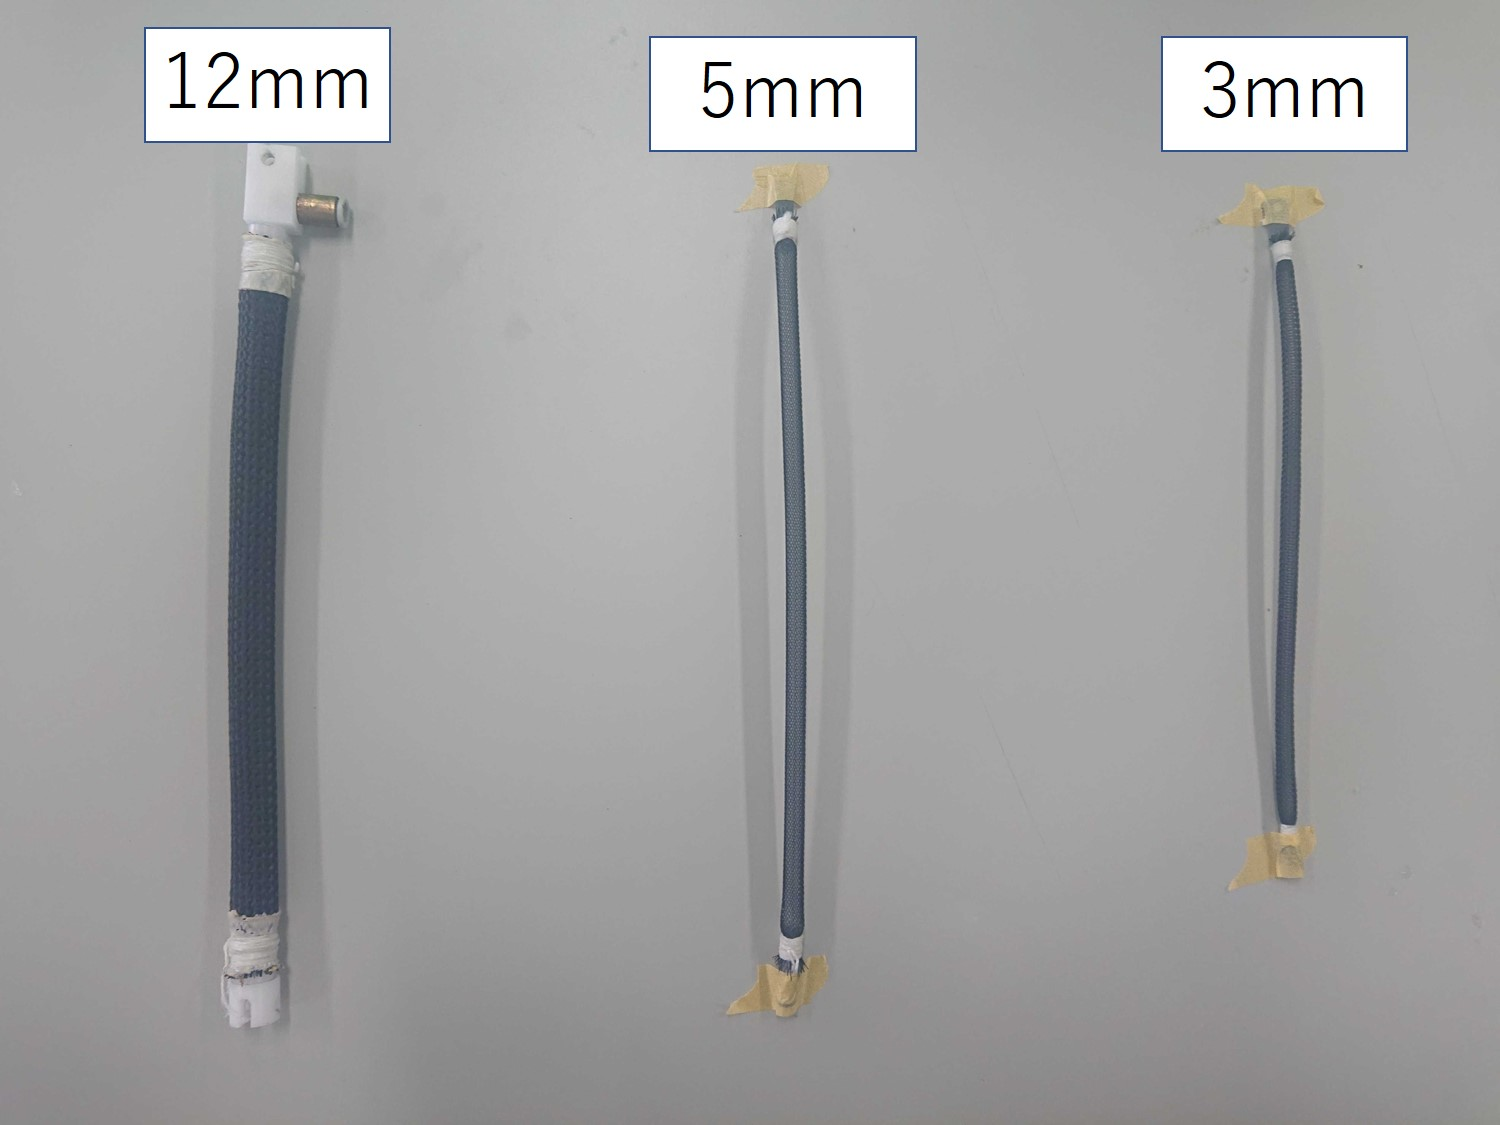
\includegraphics[scale=0.13]{mpa.JPG}
    \vspace{-4mm}
    \caption{MPAの外径}
    \label{fig:MPA}
  \end{minipage}
  \hspace{0.04\columnwidth}
  \begin{minipage}[b]{0.47\columnwidth}
    \centering
    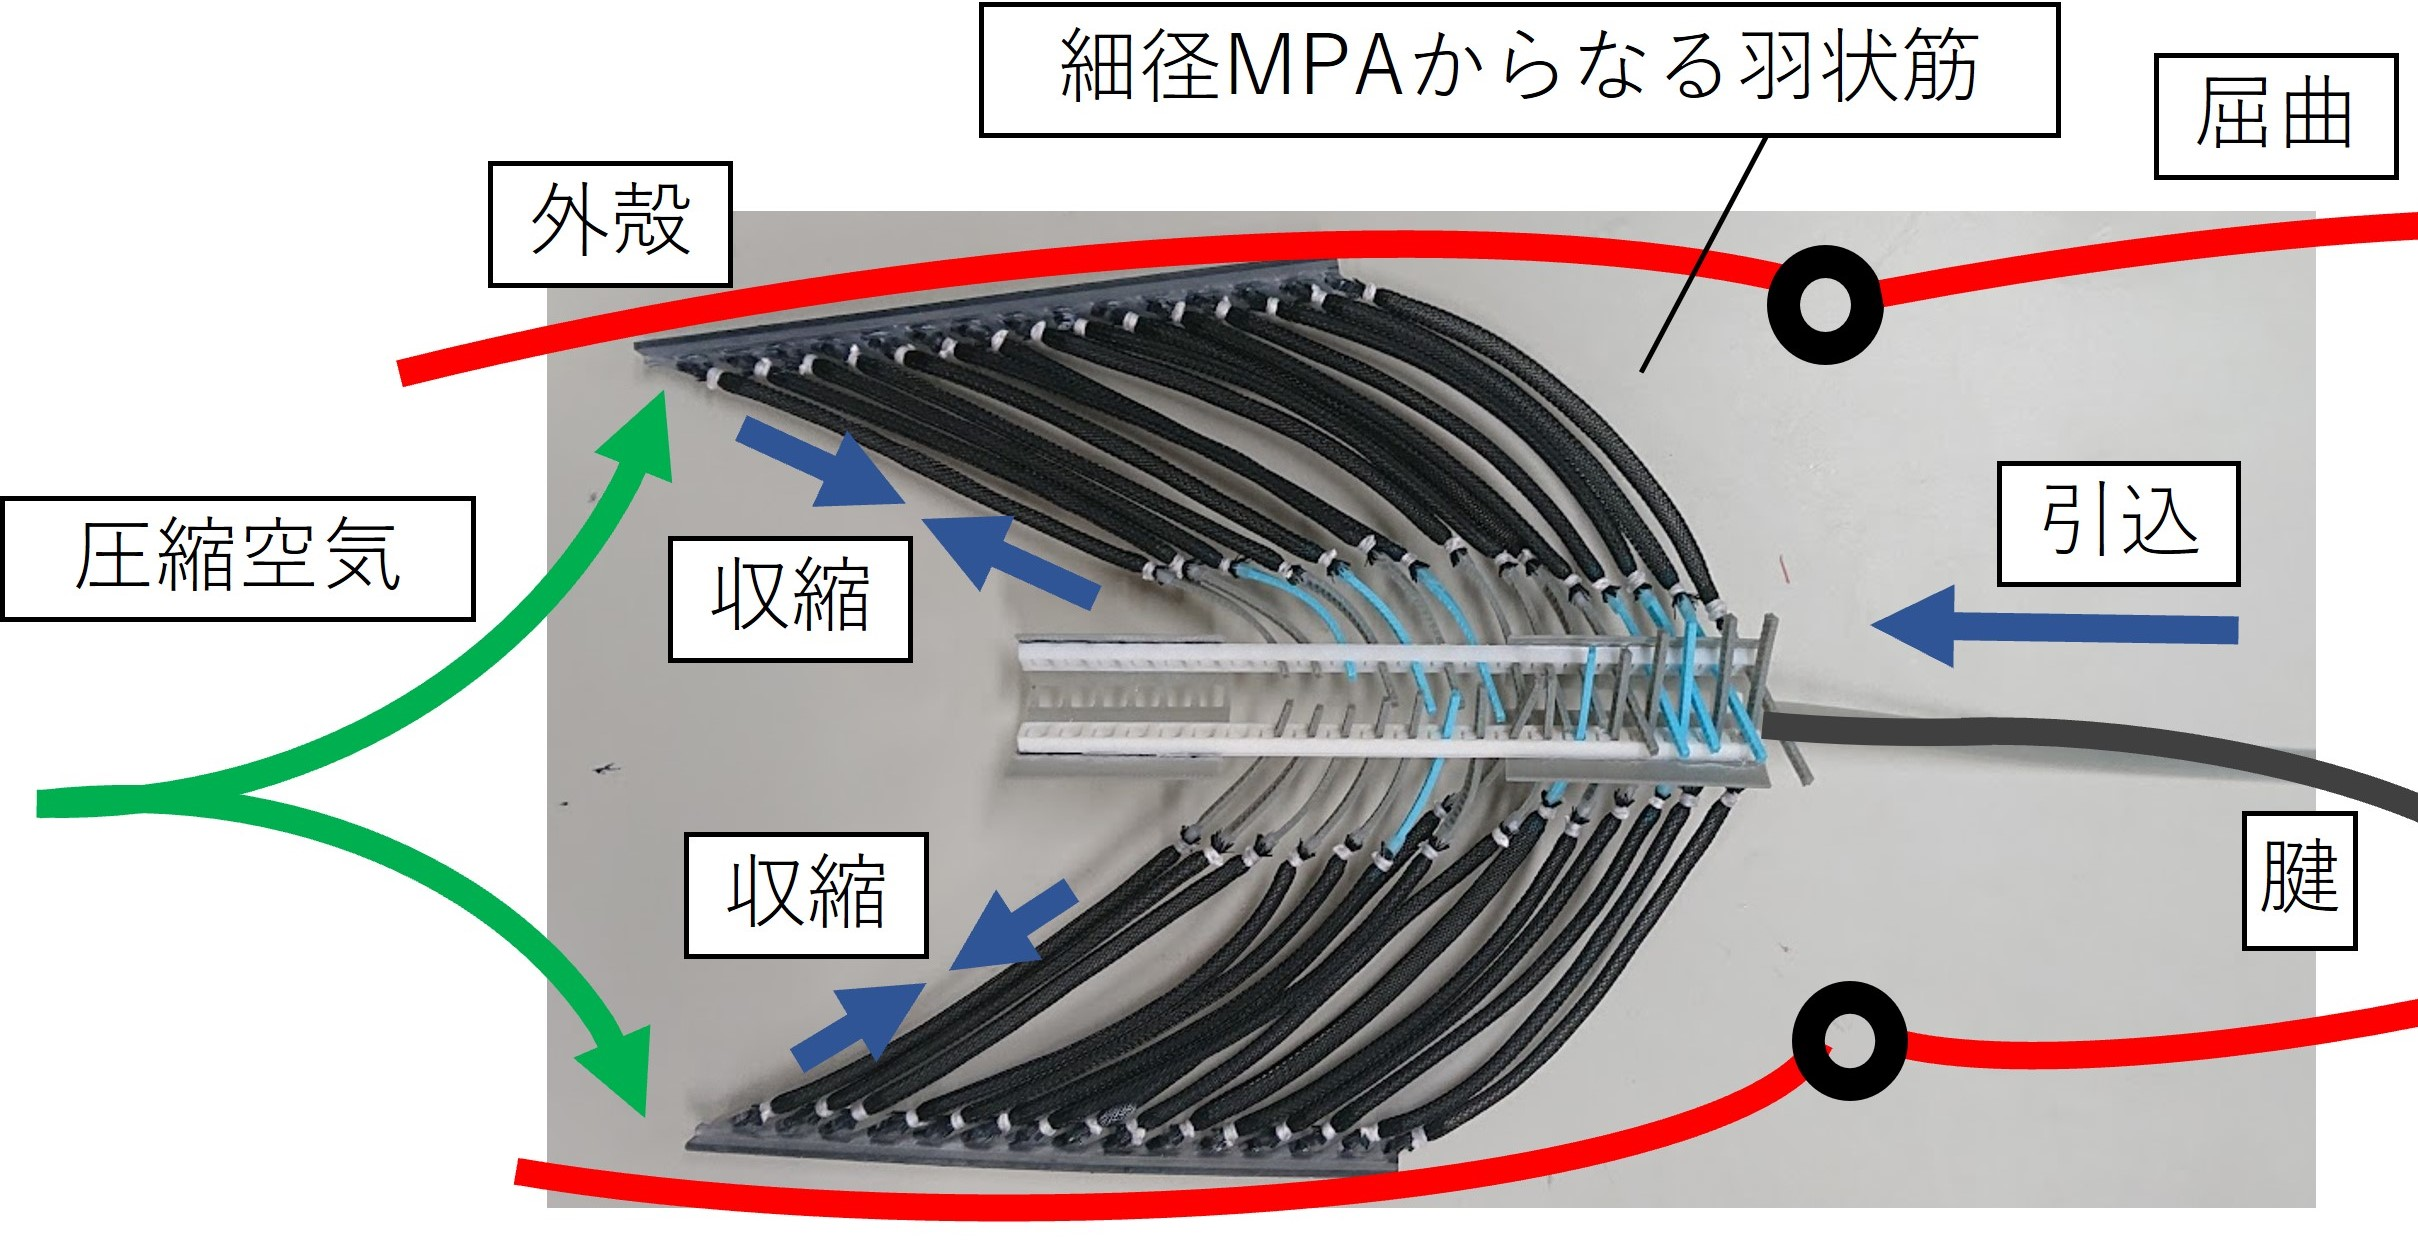
\includegraphics[scale=0.2]{mosiki.JPG}
    \vspace{-6mm}
    \caption{蟹模倣ロボット\cite{crabrobot2}}
    \label{fig:crabrobot}
  \end{minipage}
\end{figure}
\vspace*{-6mm}
\begin{figure}[H]
  \begin{minipage}[b]{0.47\columnwidth}
    \centering
    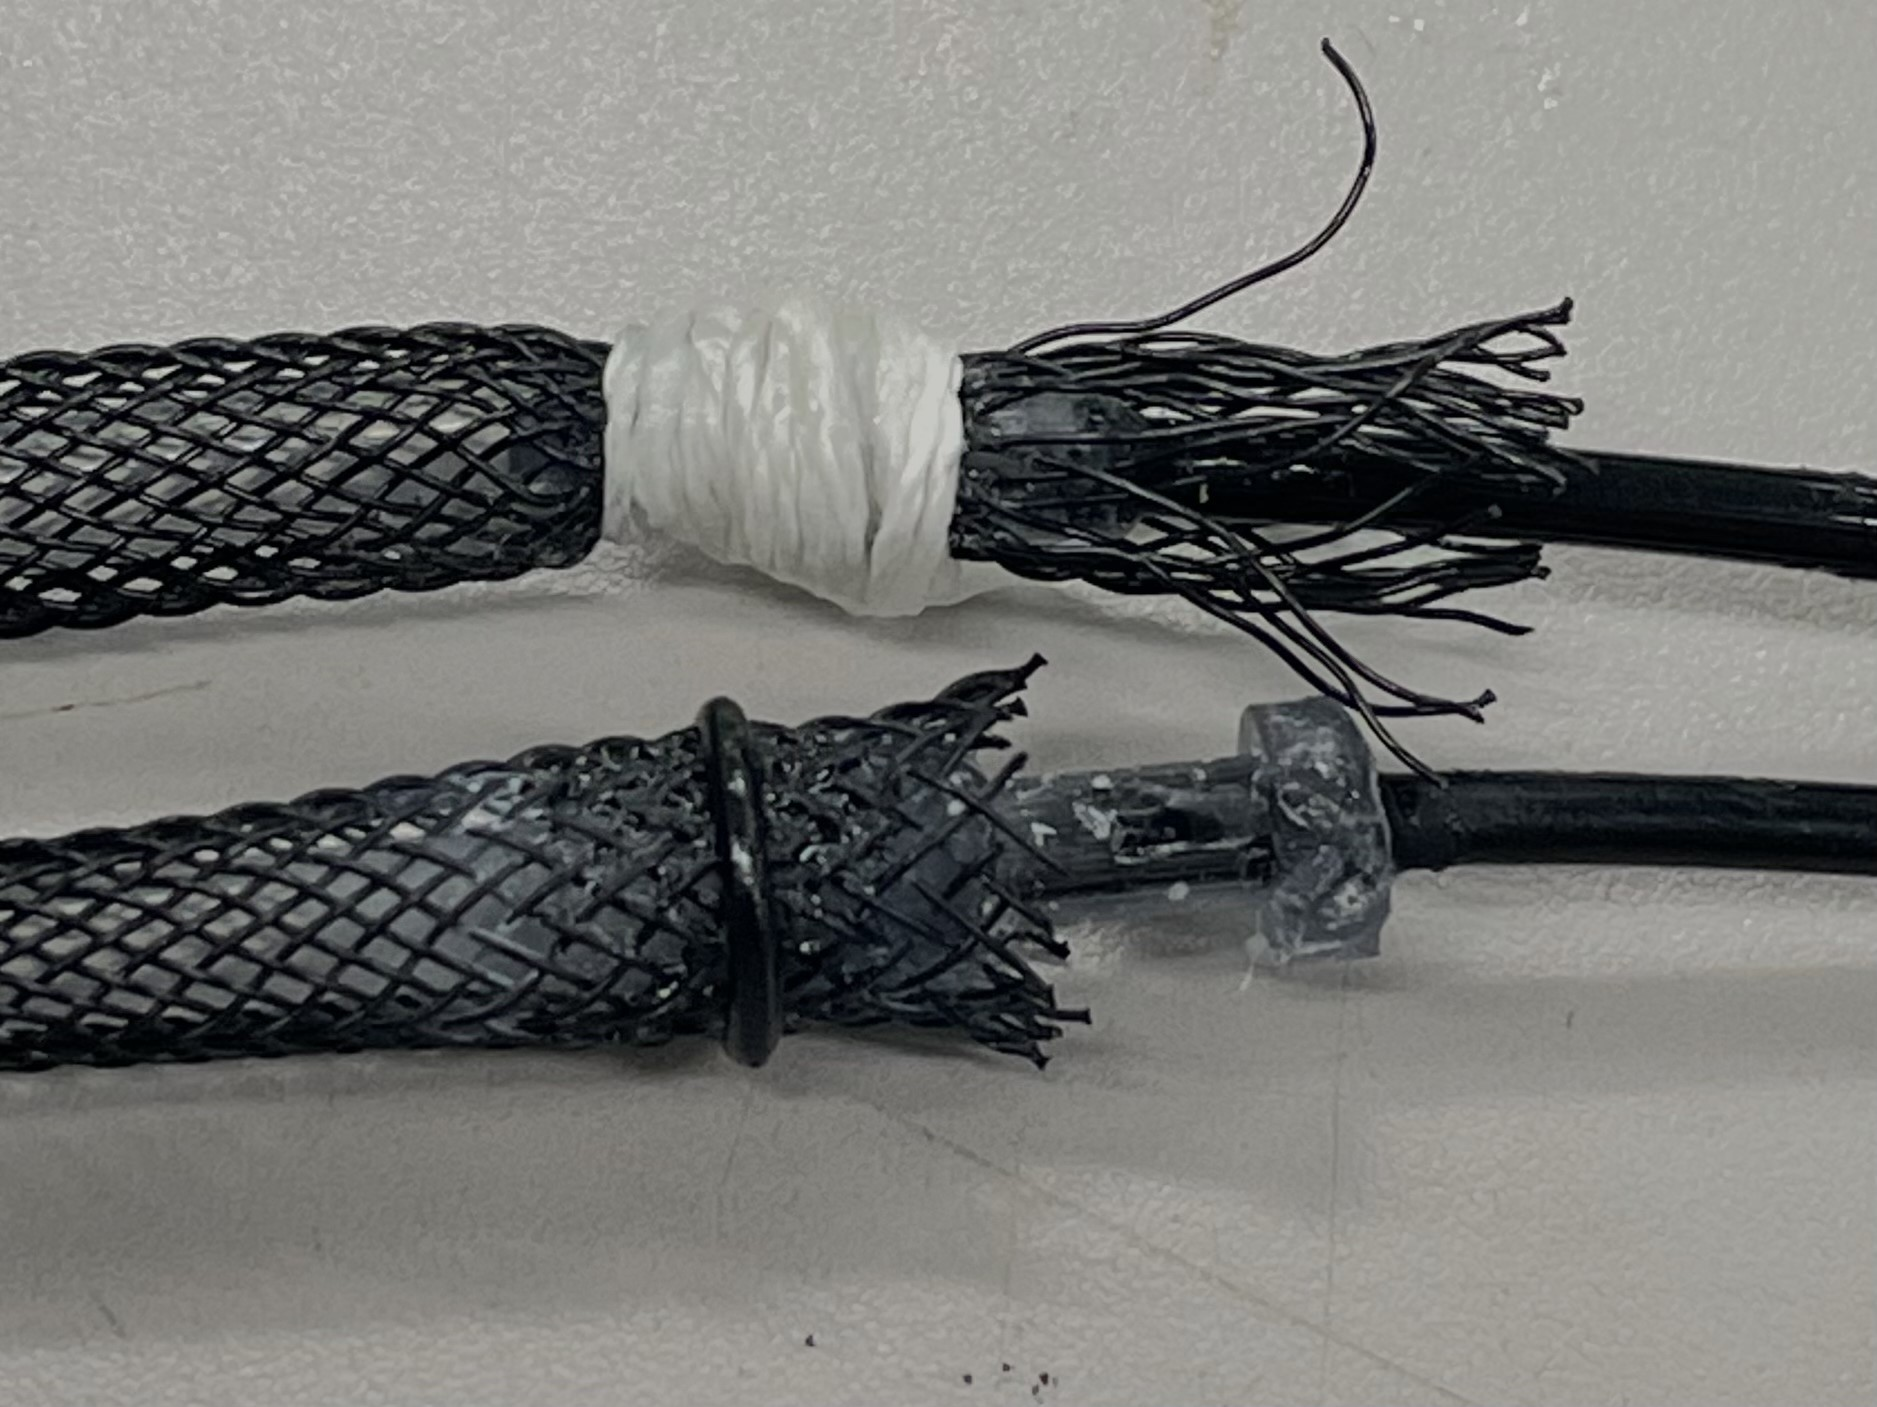
\includegraphics[scale=0.05]{mpa_oring_1.jpg}
    \vspace{-2mm}
    \caption{細径MPA}
    \label{fig:OringMPA}
  \end{minipage}
  \hspace{0.04\columnwidth}
  \begin{minipage}[b]{0.47\columnwidth}
    \centering
    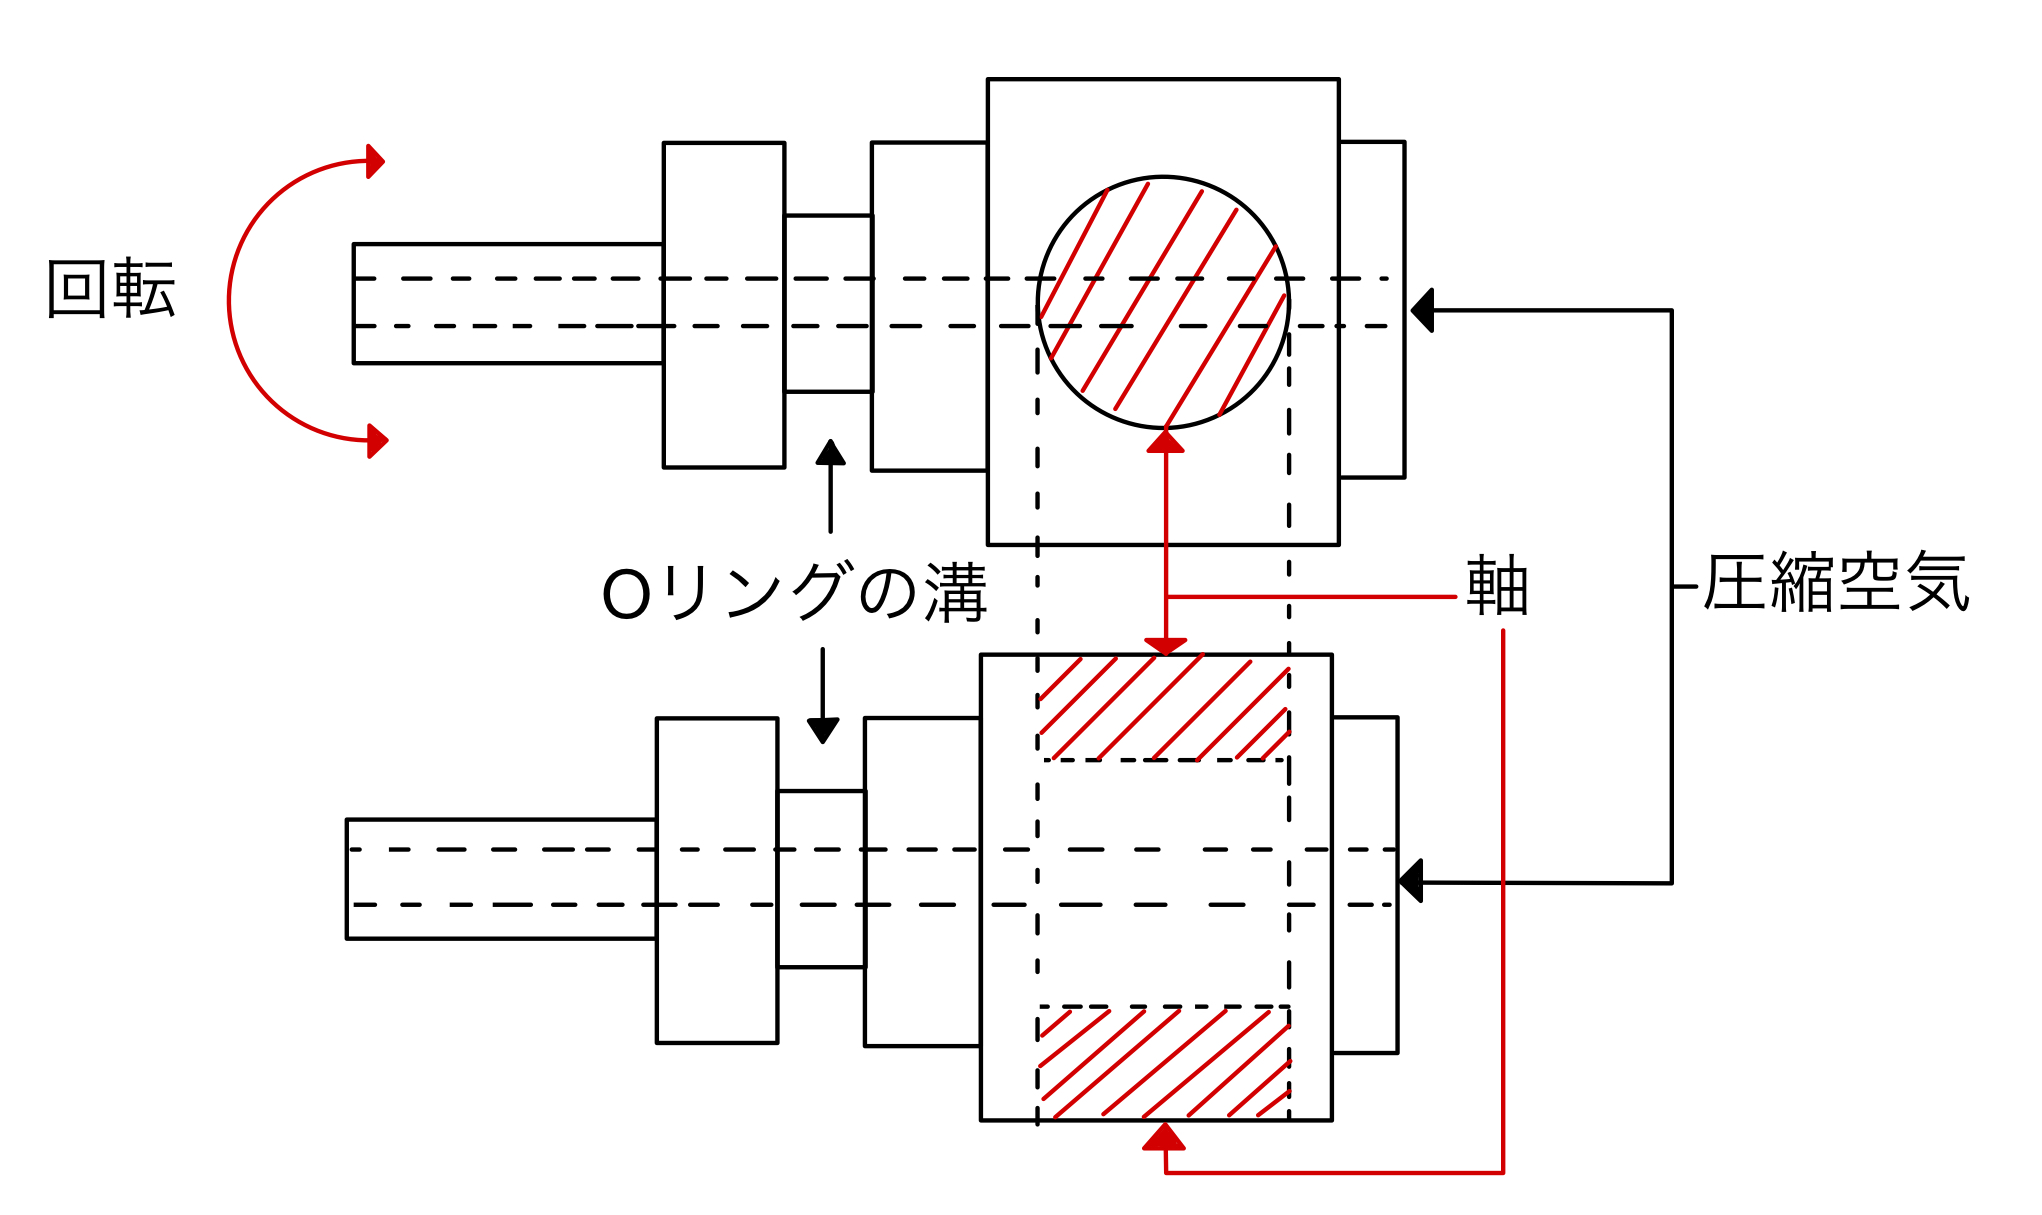
\includegraphics[scale=0.047]{MPA_irast.jpg}
    \vspace{-1mm}
    \caption{細径MPA端部部品}
    \label{fig:MPAparts}
  \end{minipage}
\end{figure}


続いて細径MPAの収縮性能向上に取り組んだ.先行研究において開発された細径MPAにおいては,折癖の影響からスリーブが多少膨らんだ状態で作成されていたため,
圧力印加時の収縮量が減少してしまっていた.本研究ではメッシュの中に直径2mmの丸棒を差し込んで固定した状態でホットプレートで加熱することで熱可逆変化させた.
折癖をとるとともにスリーブの初期直径を2mmにまで小さくすることに成功し,収縮量を向上させることができた.


最後に,細径MPAを羽状配置するために端部の部品の構造を改良した.羽状筋は収縮した際に筋肉の角度が変化するが,先行研究(図\ref{fig:crabrobot})では
根元の角度が固定されており,腱の引き込みの妨げになっていた.そこで本研究では図\ref{fig:MPAparts}の細径MPAの端部の部品を作成した.
図\ref{fig:MPAparts}の赤い斜線部の穴を回転の軸にして細径MPAの角度を自由に変化することができ,これにより細径MPA動作時に端部の部品に干渉しないことが確認できた.

%%%%%%%%%%%%%%%%%%%%%%%%%%%%%%%%%%%%%%%%%%%%%%%%%%%%%%%%%%%%%%%%%%%%%%%%%%%%%%%
\vspace*{-2mm}
\section{結言}

本稿では,外骨格生物模倣ロボットの開発をするにあたって課題となる細径MPA の作成方法と固定方法について改良を行った.
今後は羽状筋の構築,およびカニの歩脚を模したロボットの開発を行い,可動域などについて検証を行う.

%%%%%%%%%%%%%%%%%%%%%%%%%%%%%%%%%%%%%%%%%%%%%%%%%%%%%%%%%%%%%%%%%%%%%%%%%%%%%%%
\begin{thebibliography}{99}

  \bibitem{wakimoto}
  脇本修一,
  細径McKibben型人工筋の開発と用途開拓,
  計測と制御,57巻,11号,pp.812-815,2018
  
  \bibitem{crabrobot1}
  CHEN, Xi, et al. Study on the Design and Experimental Research on a Bionic Crab Robot with Amphibious Multi-Modal Movement, Journal of Marine Science and Engineering,10,12,p.1804,2022
  
  \bibitem{crabrobot2}
  中西大輔,長谷川侑大,浪花啓右,杉本靖博,
  細径空圧筋を用いた羽状筋および外骨格生物模倣ロボットの開発,ロボティクス・メカトロニクス講演会2024,2A1-L08,2024.

 \end{thebibliography}
 %%%%%%%%%%%%%%%%%%%%%%%%%%%%%%%%%%%%%%%%%%%%%%%%%%%%%%%%%%%%%%%%%%%%%%%%%%%%%%%
\end{document}